\section{Utilizzo di Butterfly}\label{utilizzo}

\subsection{Gestore Personale}

Il Gestore Personale è la componente principale di \progetto\ e si può suddividere in due sotto-componenti principali:

\begin{itemize}
    \item Interfaccia utente a sua volta divisa in
    \begin{itemize}
    	\item Interfaccia per amministratore
    	\item Interfaccia per utente normale
    \end{itemize}
    \item Message processor, che contiene la logica di business di \progetto
\end{itemize}

Il secondo punto non è di pertinenza di questo manuale (ma del \MSd), in quanto l'utente non lo usa direttamente, per cui verrà solamente discusso l'utilizzo del sistema tramite l'interfaccia utente. \par
L'inserimento della figura dell'amministratore, non presente nel \textit{Manuale Sviluppatore V1.0.0\ped{\tiny{D}}}, è giustificata in \textit{VE\_2019-04-26\ped{\tiny{D}}}.

\subsubsection{Interfaccia utente}
Le seguenti opzioni del Gestore Personale sono accessibili da ogni tipo utente, perciò anche da quelli coi privilegi di amministratore.

\paragraph{Accesso}
È possibile effettuare l'accesso all'interno del sistema tramite il link del container sul quale è in esecuzione, specificato nella configurazione effettuata precedentemente.
Per effettuare correttamente l'accesso è necessario l'inserimento del proprio ID Telegram o Email con il quale si è iscritti nel sistema.
\begin{figure}[H]
	\centering
	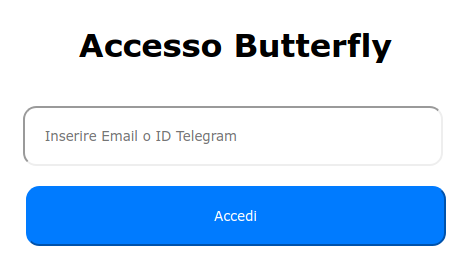
\includegraphics[width=9cm]{img/accesso_1.png}
	\caption{Form di accesso al sistema}
\end{figure}
In caso l'identificativo inserito non fosse valido, e non corrispondesse quindi a un match nel database, verrà mostrato all'utente un messaggio di errore.
\begin{figure}[H]
	\centering
	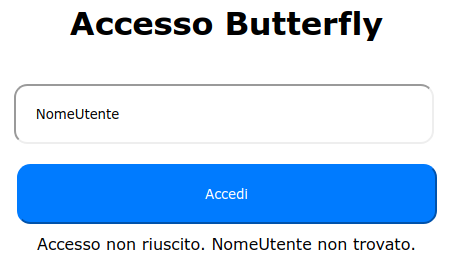
\includegraphics[width=9cm]{img/accesso_2.png}
	\caption{Messaggio di errore durante accesso al sistema}
\end{figure}

Nel caso in cui un utente cerchi di accedere ad una sezione, ma senza aver effettuato l'accesso, questo verrà rimandato alla pagina di accesso.\par
Se un utente iscritto correttamente nel sistema ha registrato precedentemente sia indirizzo Email che ID Telegram, allora può accedere utilizzando indipendentemente il primo o il secondo.
In cima alla pagina, per identificare l'utente che ha acceduto, viene mostrato l'ID Telegram o la mail con cui si ha acceduto.

\paragraph{Pannello di controllo}
Dopo aver effettuato l'accesso al sistema, si viene rimandati alla pagina relativa al pannello di controllo che contiene i comandi principali per la navigazione del sito e le operazioni che un utente può eseguire.
Le sezioni a cui si può navigare dal pannello di controllo sono:
\begin{itemize}
	\item Modifica dei propri dati
	\item Modifica delle proprie preferenze
	\item Uscita dal sistema (logout)
\end{itemize}
\begin{figure}[H]
	\centering
	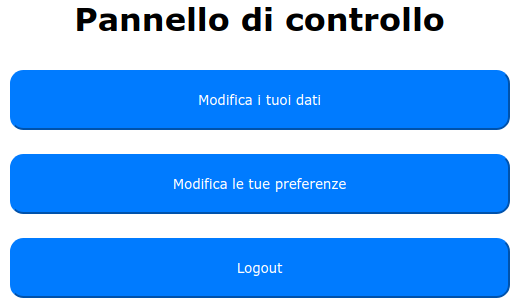
\includegraphics[width=10cm]{img/user_panel_1.png}
	\caption{Pannello di controllo per utente generico}
\end{figure}

\paragraph{Modifica preferenze}\label{preferenze}
La modifica delle preferenze è possibile solamente per utenti già iscritti ed autenticati nel sistema.
È raggiungibile tramite il pannello di controllo sotto la voce ``Modifica le tue preferenze''.
In questa sezione si possono trovare le principali impostazioni del sistema dal punto di vista dell'utente finale:
\begin{itemize}
	\item Lista dei progetti a cui si è iscritti
	\item Modifica della priorità assegnata ad un progetto che può essere:
	\begin{itemize}
        \item \textbf{Alta}: 1
        \item \textbf{Media}: 2
        \item \textbf{Bassa}: 3
    \end{itemize}
	\item Lista dei Topic (formati dall'insieme di label e keyword) disponibili e iscrizione o disiscrizione da questi, che vengono mostrati dinamicamente in base ai progetti a cui si è iscritti. L'inserimento per keyword d'interesse deve essere fatta in modo testuale e la loro divisione viene riconosciuta attraverso una ``,'' 
	\item Modifica dei progetti d'interesse (aggiunta o rimozione dei progetti dalle proprie preferenze)
	\item Inserimento dei giorni di indisponibilità da calendario
	\item Impostazione delle due piattaforme di messaggistica (Email o Telegram) su cui ricevere le notifiche. \'E possibile scegliere solo una delle due piattaforme di messaggistica
\end{itemize}
Le ``label'' non sono modificabili in quanto vengono aggiornate solamente da una componente del Gestore Personale che le memorizza quando avvengono \gloss{update} alle issue relative ai progetti.
Le ``keyword'' invece, sono formate da una lista di parole che possono essere contenute nei messaggi di push di GitLab e di cui si è interessati a ricevere notifiche.
\begin{figure}[H]
	\centering
	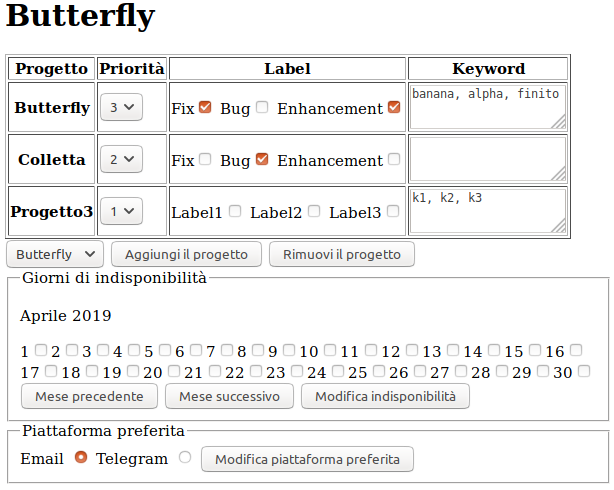
\includegraphics[width=16cm]{img/preferenze_1.png}
	\caption{Interfaccia modifica preferenze}
\end{figure}

\paragraph{Modifica dei propri dati}
La modifica dei propri dati è possibile attraverso la sezione ``Modifica i tuoi dati'' accessibile dal pannello di controllo.
Qui un utente può modificare i dati inseriti dall'amministratore in fase di registrazione.
\begin{figure}[H]
	\centering
	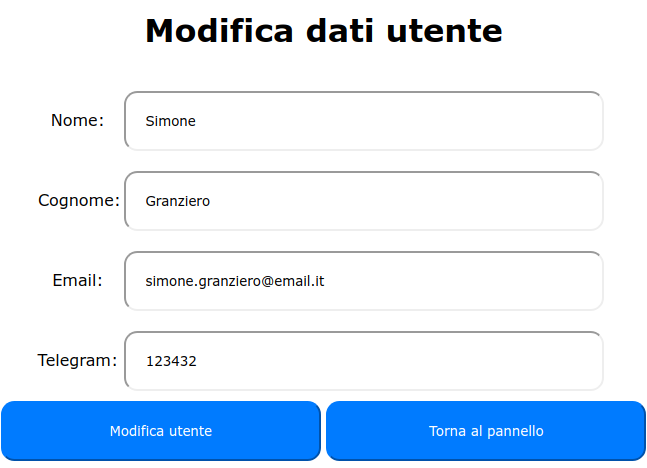
\includegraphics[width=10cm]{img/modifica_1.png}
	\caption{Modifica dei dati di un utente}
\end{figure}
Nel caso questi fossero già associati ad una persona iscritta a \progetto, verrà visualizzato un messaggio di errore. \par
Per quanto riguarda l'inserimento dell'ID Telegram, questo non deve essere nella forma \texttt{@nome\_utente}, ma bensì numerico. Per poterlo ottenere consigliamo l'utilizzo del bot Telegram ``MyIDBot\footnote{\url{https://telegram.me/storebot?start=myidbot}}'' dandogli il comando \texttt{/getid}.

\paragraph{Uscita dal sistema}
Per effettuare il logout dal sistema, cliccare sul bottone ``Logout'' presente nel pannello di controllo.

\subsubsection{Interfaccia amministratore}
All'interno dell'applicazione \progetto, gli utenti con i permessi di amministratore potranno eseguire le stesse azioni di un utente normale e in più gestire l'insieme degli utenti iscritti al sistema. Il sistema di accesso per l'utente amministratore non differisce da quello per gli altri utenti.

\paragraph{Pannello di controllo}
Dopo aver effettuato l'accesso al sistema, si viene rimandati alla pagina relativa al pannello di controllo che contiene i comandi principali per la navigazione del sito e le operazioni che un utente può eseguire.
Le sezioni a cui si può navigare dal pannello di controllo sono:
\begin{itemize}
    \item Inserimento di un nuovo utente
    \item Rimozione di un utente
    \item Visualizzazione degli utenti iscritti
    \item Rimozione di un progetto
    \item Visualizzazione dei progetti
    \item Modifica dei propri dati
    \item Modifica delle proprie preferenze
	\item Uscita dal sistema (logout)
\end{itemize}
\begin{figure}[H]
    \centering
    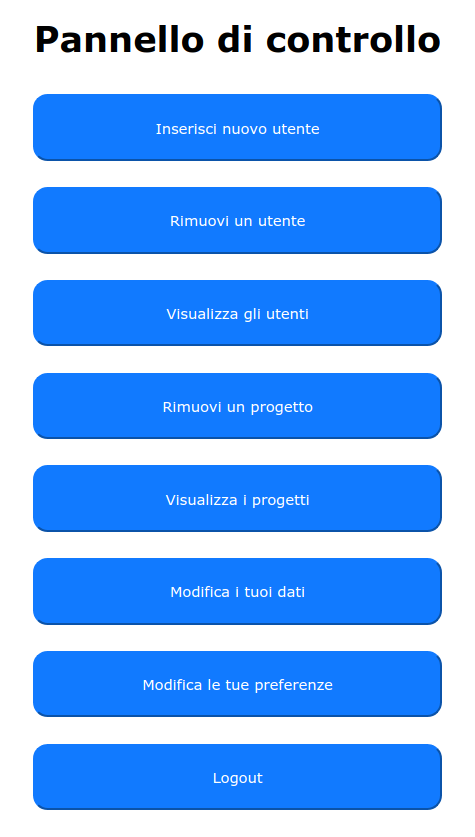
\includegraphics[width=10cm]{img/admin_panel_1.png}
    \caption{Pannello di controllo per utente con privilegi di amministratore}
\end{figure}

\paragraph{Iscrizione a Butterfly}\label{Iscrizione}
L'iscrizione di un nuovo utente al sistema \progetto\ è permessa solamente all'utente amministratore.
La sezione di inserimento di un nuovo utente è raggiungibile dal pannello di controllo e prevede l'inserimento dei seguenti dati:
\begin{itemize}
	\item Nome
	\item Cognome
	\item Email
	\item Telegram
\end{itemize}
\begin{figure}[H]
	\centering
	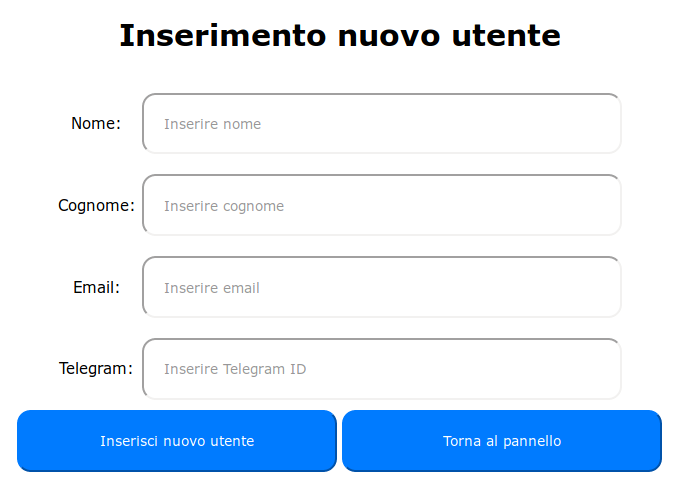
\includegraphics[width=13cm]{img/inserimento_1.png}
	\caption{Interfaccia inserimento nuovo utente}
\end{figure}

È necessario inserire almeno un campo a scelta tra Email e Telegram.
Nel caso questi fossero già associati ad un utente iscritto a \progetto\ verrà visualizzato un messaggio di errore.

\paragraph{Rimozione di un utente}\label{Rimozione}
Viene data la possibilità di rimuovere un utente dal sistema solamente all'amministratore.
La rimozione è possibile attraverso la sezione ``Rimuovi un utente'' accessibile dal pannello di controllo.
\begin{figure}[H]
	\centering
	
\includegraphics[width=12cm]{img/rimozione_1.png}
	\caption{Interfaccia rimozione di un utente}
\end{figure}

\paragraph{Visualizzazione utenti} \label{VisUtenti}
Un utente amministratore ha la possibilità di vedere la lista di tutti gli utenti iscritti al sistema e i relativi progetti a cui sono interessati.
Per ogni progetto viene inoltre riportata la priorità che ha per l'utente, le labels e la keywords d'interesse.
La visualizzazione avviene attraverso la sezione ``Visualizza gli utenti'' accessibile dal pannello di controllo.
\begin{figure}[H]
	\centering
	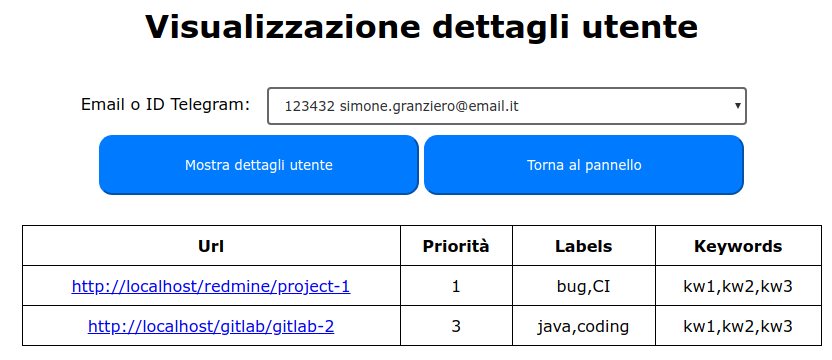
\includegraphics[width=12cm]{img/user_details.png}
	\caption{Interfaccia visualizzazione degli utenti}
\end{figure}

\paragraph{Rimozione di un progetto}
I progetti provenienti da GitLab o Redmine vengono aggiunti in automatico al sistema e la loro gestione (intesa come creazione e modifica) non è competenza degli utenti. Perciò i progetti possono solo essere aggiunti o rimossi dalle preferenze di un utente, oppure rimossi completamente dal sistema nel momento in cui questi, ad esempio, vengono chiusi nelle relative applicazioni di provenienza. \par
Per rimuovere un progetto dal sistema, l'interfaccia dell'amministratore possiede un'apposita pagina chiamata ``Rimuovi un  progetto'' dove è possibile selezionare i progetti da rimuovere.
\begin{figure}[H]
    \centering
	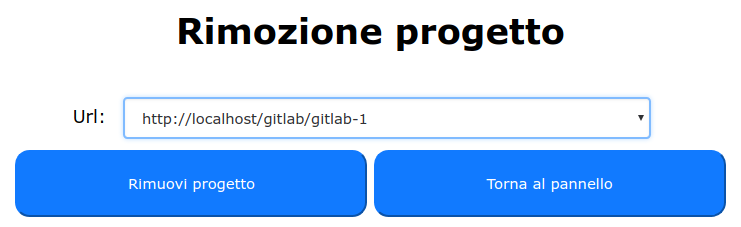
\includegraphics[width=12cm]{img/rimozioneprog.png}
	\caption{Interfaccia rimozione di un progetto }
\end{figure}

\paragraph{Visualizzazione dei progetti}
Un utente amministratore ha la possibilità di vedere la lista di tutti i progetti presenti nel sistema. Di ognuno viene mostrata la url identificativa, il nome, l'applicazione di provenienza e i topics rilevati relativi al progetto.
La visualizzazione avviene attraverso la sezione ``Visualizza i progetti'' accessibile dal pannello di controllo.
\begin{figure}[H]
	\centering
	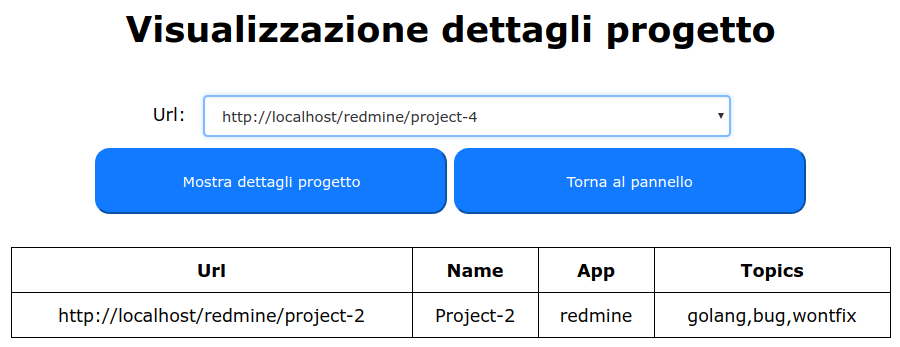
\includegraphics[width=12cm]{img/visualizzaprog.png}
	\caption{Interfaccia visualiazzione dei progetti}
\end{figure}


\subsection{API Rest}\label{APIRest}
\newcommand{\homeUrl}{home\_url}

Per la gestione delle risorse di \progetto\ abbiamo utilizzato lo standard architetturale delle API Rest.
Nelle sezioni successive viene descritto come interagire con le API fornite dal sistema.
Il \gloss{root path} sottinteso sarà sempre \texttt{\homeUrl/api/v1/}.
Ad esempio, per effettuare la GET dell'user \texttt{@user1}, l'indirizzo sarà:
\begin{center}
    \texttt{GET \homeUrl/api/v1/user/@user1}
\end{center}

\subsubsection{User}

\texttt{User} è la risorsa utente.
È possibile visualizzare, aggiungere, modificare o rimuovere gli utenti tramite una semplice
richiesta HTTP.

\paragraph{Visualizzazione}
È possibile visualizzare i dati di un utente tramite la richiesta
    \begin{center}
        \texttt{GET  /user/<id>}
    \end{center}

    \subparagraph{Esempio di input}
    Un esempio di richiesta è
        \begin{center}
            \texttt{GET  /user/abcd@bc.it}
        \end{center}
    senza alcun dato nel \gloss{payload} della richiesta.

    \subparagraph{Esempio di output}
    In caso la richiesta vada a buon fine, un esempio di output è
    \begin{lstlisting}[language = json]
{
    "_id": {
        "$oid": "5cd07bb9c331755af7f5ea00"
    },
    "name": "Mattia",
    "surname": "Cruciani",
    "email": "abcd@bc.it",
    "telegram": "1234",
    "admin": false,
    "preference": "email",
    "irreperibilita": [
        {
            "$date": "2018-12-05"
        },
        {
            "$date": "2019-04-08"
        },
        {
            "$date": "2019-04-15"
        },
        {
            "$date": "2019-04-07"
        },
        {
            "$date": "2019-06-07"
        },
        {
            "$date": "2019-06-08"
        },
        {
            "$date": "2019-06-09"
        }
    ],
    "projects": [
        {
            "url": "http://localhost/gitlab/gitlab-2",
            "priority": 2,
            "topics": [
                "java",
                "coding",
                "criptovaluta"
            ],
            "keywords": [
                "kw1",
                "kw2",
                "kw3"
            ]
        }
    ]
}
    \end{lstlisting}

    Nel caso l'utente richiesto non venga trovato, verrà restituito il seguente messaggio
    \begin{lstlisting}[language = json]
{
    "error": "Utente inesistente."
}
    \end{lstlisting}

\paragraph{Inserimento}
È possibile inserire un nuovo utente tramite la richiesta:
    \begin{center}
        \texttt{POST /user}
    \end{center}

È inoltre possibile dare i seguenti campi di tipo stringa alla richiesta, per aggiungere in fase di creazione i dati:
\begin{itemize}[noitemsep]
    \item \texttt{name}
    \item \texttt{surname}
    \item \texttt{telegram}
    \item \texttt{email}
\end{itemize}
Almeno uno tra i campi \texttt{Email} e \texttt{ID Telegram} vanno fornite insieme al payload.

    \subparagraph{Esempio di input}
    Un esempio di richiesta è
        \begin{center}
            \texttt{POST  /user}
        \end{center}
    con i seguenti dati nel corpo della richiesta
    \begin{lstlisting}[language = json]
{
    "name": "Matteo",
    "surname": "Marchiori",
    "email": "matteo.marchiori97@gmail.com",
    "telegram": "123456"
}
    \end{lstlisting}


    \subparagraph{Esempio di output}
    In caso la richiesta vada a buon fine, verrà restituito il seguente messaggio
    \begin{lstlisting}[language = json]
{
    "ok": "Utente inserito correttamente"
}
    \end{lstlisting}

    Nel caso l'utente da inserire esista già, verrà restituito il seguente messaggio
    \begin{lstlisting}[language = json]
{
    "error": "L'utente inserito esiste già."
}
    \end{lstlisting}

    Nel caso non vengano inseriti almeno email o telegram, verrà restituito il seguente messaggio
    \begin{lstlisting}[language = json]
{
    "error": "Si prega di inserire almeno email o telegram per inserire l'utente."
}
    \end{lstlisting}

\paragraph{Modifica}

È possibile modificare un utente tramite la richiesta
\begin{center}
    \texttt{PUT /user/<id>}
\end{center}

È possibile dare i seguenti campi di tipo stringa alla richiesta, per aggiungere in fase di modifica i dati:
\begin{itemize}[noitemsep]
    \item \texttt{name}
    \item \texttt{surname}
    \item \texttt{telegram}
    \item \texttt{email}
\end{itemize}

    \subparagraph{Esempio di input}
    Un esempio di richiesta è
    \begin{center}
	    \texttt{PUT /user/1234}
    \end{center}
    con i seguenti dati nel corpo della richiesta
	\begin{lstlisting}[language = json]
{
    "name": "Marco",
    "surname": "Rossi",
    "telegram": "1235"
}
    \end{lstlisting}

    \subparagraph{Esempio di output}
    In caso la richiesta vada a buon fine, verrà restituito il seguente messaggio
	\begin{lstlisting}[language = json]
{
    "ok": "Utente modificato correttamente"
}
	\end{lstlisting}

	In caso non vengano forniti almeno Email o ID Telegram, verrà restituito il seguente messaggio
	\begin{lstlisting}[language = json]
{
    "error": "Si prega di inserire almeno email o telegram per modificare l'utente."
}
	\end{lstlisting}

	In caso almeno uno degli identificativi forniti coincida con quello di un altro utente, verrà restituito il seguente messaggio
	\begin{lstlisting}[language = json]
{
    "error": "I dati inseriti confliggono con altri già esistenti."
}
	\end{lstlisting}

\paragraph{Rimozione}

È possibile rimuovere un utente dal sistema \progetto\ con la richiesta
\begin{center}
    \texttt{DELETE /user/<id>}
\end{center}

Se il campo \texttt{<id>} corrisponde a un ID presente nel sistema, esso verrà rimosso.

    \subparagraph{Esempio di input}
    Un esempio di richiesta è
    \begin{center}
        \texttt{DELETE  /user/abcd@bc.it}
    \end{center}
    senza alcun dato nel \gloss{payload} della richiesta.

    \subparagraph{Esempio di output}
    In caso la richiesta vada a buon fine, verrà restituito il seguente messaggio
	\begin{lstlisting}[language = json]
{
    "ok": "Utente rimosso correttamente"
}
	\end{lstlisting}


\paragraph{Riepilogo}

\begin{table}[H]
    \begin{paddedtablex}[1.3]{\textwidth}{cYY}
        \thead{Metodo HTTP} & \thead{URI} & \thead{Action}\\\toprule
        \texttt{GET} & \texttt{/user/<id>} & Restituisce un payload in JSON dell'utente che corrisponde a \texttt{<id>}\\
        \texttt{POST} & \texttt{/user} & Inserisce un nuovo utente. È necessario fornire uno tra i campi telegram o email\\
        \texttt{PUT} & \texttt{/user/<id>} & Modifica l'utente corrispondente a \texttt{<id>} con i campi passati nella richiesta\\
        \texttt{DELETE} & \texttt{/user/<id>} & Elimina l'utente corrispondente a \texttt{<id>} dal sistema\\
        \bottomrule
    \end{paddedtablex}
    \caption{Riepilogo delle Rest API per la risorsa User}
\end{table}


\subsubsection{Project}
Project è la risorsa relativa ai progetti. È possibile visualizzare o rimuovere i progetti tramite una semplice richiesta HTTP.

\paragraph{Visualizzazione}
È possibile visualizzare i progetti tramite la richiesta
    \begin{center}
        \texttt{GET /project/<id>}
    \end{center}
Se il campo \texttt{<id>} corrisponde a un progetto, verranno mostrati i dati relativi a tale progetto.

    \subparagraph{Esempio di input}
    Un esempio di richiesta è
        \begin{center}
            \texttt{GET /project/http://localhost/gitlab/gitlab-2}
        \end{center}
    senza alcun dato nel \gloss{payload} della richiesta.

    \subparagraph{Esempio di output}
    In caso la richiesta vada a buon fine, un esempio di output è
    \begin{lstlisting}[language = json]
{
    "_id": {
        "$oid": "5cd1b509c331756598e9c00b"
    },
    "url": "http://localhost/gitlab/gitlab-2",
    "name": "Gitlab-2",
    "app": "gitlab",
    "topics": [
        "java",
        "coding",
        "enhancement",
        "bug"
    ]
}
	\end{lstlisting}

	In caso il progetto richiesto non esista, verrà restituito il seguente messaggio
    \begin{lstlisting}[language = json]
{
    "error": "Progetto inesistente."
}
	\end{lstlisting}


\paragraph{Rimozione}

È possibile rimuovere un progetto dal sistema Butterfly con la richiesta
\begin{center}
    \texttt{DELETE /project/<id>}
\end{center}

Se il campo \texttt{<id>} corrisponde a un progetto, esso verrà rimossa dal sistema.

    \subparagraph{Esempio di input}
    Un esempio di richiesta è
    \begin{center}
	    \texttt{DELETE /project/http://localhost/gitlab/gitlab-2}
    \end{center}
    senza alcun dato nel \gloss{payload} della richiesta.

    \subparagraph{Esempio output}
    In caso la richiesta vada a buon fine, verrà restituito il seguente messaggio
    \begin{lstlisting}[language = json]
{
    "ok": "Progetto rimosso correttamente"
}
    \end{lstlisting}

\paragraph{Riepilogo}

\begin{table}[H]
    \begin{paddedtablex}[1.3]{\textwidth}{cYY}
        \thead{Metodo HTTP} & \thead{URI} & \thead{Action}\\\toprule
        \texttt{GET} & \texttt{/project/<id>} & Restituisce un payload in JSON del progetto corrispondente a \texttt{<id>}\\
        \texttt{DELETE} & \texttt{/project/<id>} & Elimina il progetto corrispondente a \texttt{<id>} dal sistema \\
        \bottomrule
    \end{paddedtablex}
    \caption{Riepilogo delle Rest API per la risorsa Project}
\end{table}


\subsubsection{Preference}

\texttt{Preference} è la risorsa preferenza.
È possibile modificare le preferenze degli utenti tramite questa risorsa.

\paragraph{Inserimento}
È possibile inserire un nuovo progetto tra le preferenze tramite la richiesta:
    \begin{center}
        \texttt{POST /preference}
    \end{center}

È inoltre richiesto dare i seguenti campi di tipo stringa alla richiesta, per aggiungere in fase di creazione i dati:
\begin{itemize}[noitemsep]
    \item \texttt{user}
    \item \texttt{project}
\end{itemize}

    \subparagraph{Esempio di input}
    Un esempio di richiesta è
        \begin{center}
            \texttt{POST  /preference}
        \end{center}
    con i seguenti dati nel corpo della richiesta
    \begin{lstlisting}[language = json]
{
    "user": "1234",
    "project": "http://localhost/redmine/project-2"
}
    \end{lstlisting}


    \subparagraph{Esempio di output}
    In caso la richiesta vada a buon fine, verrà restituito il seguente messaggio
    \begin{lstlisting}[language = json]
{
    "ok": "Preferenza aggiunta correttamente"
}
    \end{lstlisting}

    Nel caso il progetto esista già tra le preferenze, o non esista l'utente specificato, verrà restituito il seguente messaggio
    \begin{lstlisting}[language = json]
{
    "error": "Progetto già presente o utente inesistente."
}
    \end{lstlisting}

    Nel caso non venga specificato il progetto, verrà restituito il seguente messaggio
    \begin{lstlisting}[language = json]
{
    "error": "Nessun progetto selezionato o progetto inesistente."
}
    \end{lstlisting}


\paragraph{Modifica}

È possibile modificare le preferenze di un utente tramite la richiesta
\begin{center}
    \texttt{PUT /preference/<id>}
\end{center}

Le preferenze hanno i seguenti tipi:
\begin{itemize}[noitemsep]
    \item \texttt{topics}
    \item \texttt{irreperibilita}
    \item \texttt{piattaforma}
\end{itemize}

Il tipo di preferenza va indicato nel payload usando il campo ``tipo''.

In base al tipo di preferenza è possibile dare i seguenti campi di tipo stringa alla richiesta, per aggiungere in fase di modifica i dati:

\begin{itemize}[noitemsep]
    \item \texttt{topics}
    \begin{itemize}
        \item \texttt{project}
        \item \texttt{priority}
        \item \texttt{topics}
        \item \texttt{keywords}
    \end{itemize}
    \item \texttt{irreperibilita}
    \begin{itemize}
        \item \texttt{giorni}
    \end{itemize}
    \item \texttt{piattaforma}
    \begin{itemize}
        \item \texttt{platform}
    \end{itemize}
\end{itemize}

    \subparagraph{Esempio di input}
    Un esempio di richiesta è
    \begin{center}
	    \texttt{PUT /preference/1234}
    \end{center}
    con i seguenti dati nel corpo della richiesta
	\begin{lstlisting}[language = json]
{
    "tipo": "topics",
    "project": "http://localhost/redmine/project-2",
    "priority": "2",
    "topics": "['bug','feature','banana']",
    "keywords": "['keyword','42']"
}
    \end{lstlisting}

    Un esempio per l'irreperibilità è
    \begin{center}
	    \texttt{PUT /preference/1234}
    \end{center}
    con i seguenti dati nel corpo della richiesta
	\begin{lstlisting}[language = json]
{
    "tipo": "irreperibilita",
    "giorni": "['2019-05-25','2019-05-26','2019-06-01']"
}
    \end{lstlisting}

    Invece un esempio per modificare la piattaforma preferita di ricezione dei messaggi è
    \begin{center}
	    \texttt{PUT /preference/1234}
    \end{center}
    con i seguenti dati nel corpo della richiesta
	\begin{lstlisting}[language = json]
{
    "tipo": "piattaforma",
    "platform": "email"
}
    \end{lstlisting}

    \subparagraph{Esempio di output}
    In caso la richiesta vada a buon fine, verrà restituito il seguente messaggio
	\begin{lstlisting}[language = json]
{
    "ok": "Preferenza modificata correttamente"
}
	\end{lstlisting}

	Nel caso si stia cercando di impostare la piattaforma preferita non avendo registrato l'account verrà restituito uno dei seguenti messaggi
	\begin{lstlisting}[language = json]
{
    "error": "Telegram non presente nel sistema."
}
	\end{lstlisting}

	oppure

	\begin{lstlisting}[language = json]
{
    "error": "Email non presente nel sistema."
}
	\end{lstlisting}

\paragraph{Rimozione}

È possibile rimuovere un progetto dalle preferenze di un utente con la richiesta
\begin{center}
    \texttt{DELETE /preference/<id>}
\end{center}

Se il campo \texttt{<id>} corrisponde a un utente, il progetto verrà rimosso dalle sue preferenze.

    \subparagraph{Esempio di input}
    Un esempio di richiesta è
    \begin{center}
	    \texttt{DELETE /preference/1234}
    \end{center}
    con i seguenti dati nel corpo della richiesta
	\begin{lstlisting}[language = json]
{
    "project": "http://localhost/redmine/project-2"
}
    \end{lstlisting}

    \subparagraph{Esempio output}
    In caso la richiesta vada a buon fine, verrà restituito il seguente messaggio
    \begin{lstlisting}[language = json]
{
    "ok": "Preferenza rimossa correttamente."
}
    \end{lstlisting}

    In caso non venga fornito un progetto nella richiesta, verrà restituito il messaggio
    \begin{lstlisting}[language = json]
{
    "error": "Nessun progetto selezionato o progetto inesistente."
}
    \end{lstlisting}

    In caso l'utente non abbia il progetto specificato tra le preferenze o non esista l'utente specificato verrà restituito il messaggio
    \begin{lstlisting}[language = json]
{
    "error": "Progetto non presente nelle preferenze o utente inesistente."
}
    \end{lstlisting}

\paragraph{Riepilogo}

\begin{table}[H]
    \begin{paddedtablex}[1.3]{\textwidth}{cYY}
        \thead{Metodo HTTP} & \thead{URI} & \thead{Action}\\\toprule
        \texttt{POST} & \texttt{/preference} & Aggiunge la preferenza all'utente specificato nella richiesta con i campi passati nella richiesta\\
        \texttt{PUT} & \texttt{/preference/<id>} & Modifica la preferenza dell'utente corrispondente a \texttt{<id>} con i campi passati nella richiesta\\
        \texttt{DELETE} & \texttt{/preference/<id>} & Rimuove la preferenza dell'utente corrispondente a \texttt{<id>}\\
        \bottomrule
    \end{paddedtablex}
    \caption{Riepilogo delle Rest API per la risorsa Preference}
\end{table}


\newpage

\subsection{Piattaforma di messaggistica}

\subsubsection{Email}

Per ricevere i messaggi di Butterfly tramite Email, è sufficiente fornire tramite l'interfaccia del Gestore Personale l'Email sulla quale si vuole ricevere la notifica.

\begin{figure}[H]
	\centering
	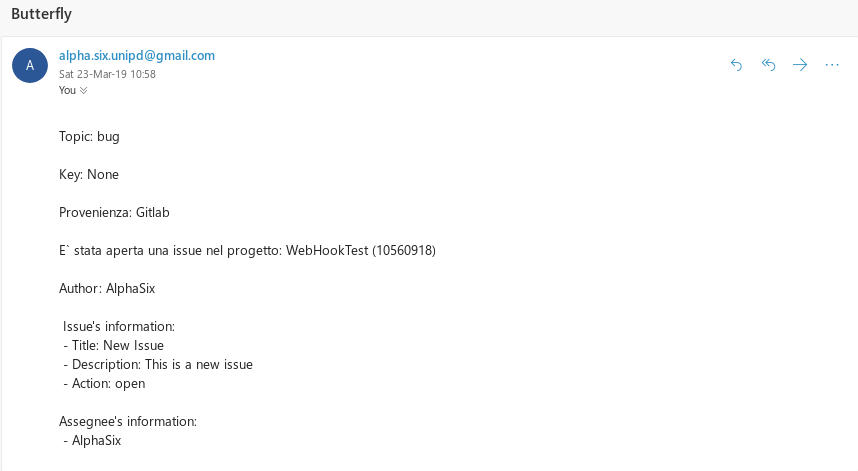
\includegraphics[width=\textwidth]{img/notifica_email_1.png}
	\caption{Formato dell' Email ricevuta da un utente finale}
\end{figure}

\subsubsection{Telegram}

Per ricevere le notifiche via Telegram, è necessario fare un passaggio addizionale: va fornita l'autorizzazione al bot per poter inviare messaggi agli utenti.
Il bot è raggiungibile al seguente link:
\begin{center}
    \url{http://t.me/ButterflyBot}
\end{center}

Dare il comando \texttt{/start} per dare l'autorizzazione di inoltro dei messaggi al bot.
È necessario inoltre aggiungere tramite l'interfaccia del Gestore Personale il proprio account Telegram.
In qualsiasi momento sarà possibile bloccare il bot in caso non si vogliano più ricevere messaggi relativi a Butterfly su Telegram, tramite le funzionalità dell'applicazione.
\begin{figure}[H]
	\centering
	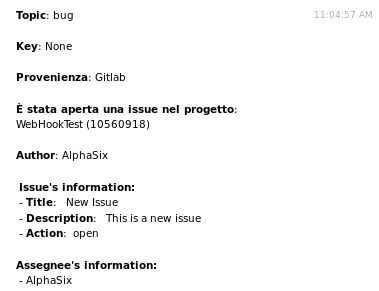
\includegraphics[width=9cm]{img/notifica_telegram_1.png}
	\caption{Formato del messaggio Telegram ricevuto da un utente finale}
\end{figure}
Nel caso in cui si volesse utilizzare un altro bot, i passaggi da seguire possono essere trovati sulla pagina apposita della documentazione di Telegram\footnote{\url{https://core.telegram.org/bots}}.
Per comunicare con questo bisogna modificare la variabile di ambiente \texttt{BUTTERFLY\_CONSUMER\_TELEGRAM\_BOT} che rappresenta il \texttt{token} univoco del nuovo bot, come descritto in \S\ref{var_consumer}.
